%!TEX root = ../graduate-work.tex

\section{Предлагаемый метод}
% Здесь надо декомпозировать большую задачу из постановки на подзадачи и продолжать этот процесс, пока подзадачи не станут достаточно простыми, чтобы их можно было бы решить напрямую (например, поставив какой-то эксперимент или доказав теорему) или найти готовое решение.

% \begin{theorem}\label{theorem1}

% \begin{itemize}
%     \item[1)] Гомоморфный образ группы
%     \item[2)] Что во имя коммунизма
%     \item[3)] Изоморфен фактор-группе
%     \item[4)] По ядру гомоморфизма
% \end{itemize}
% \end{theorem}
% \begin{proof}
%     Доказательство оставляем читателю.
% \end{proof}
\subsection{Общая идея подхода}

Задачу автоматической оценки качества радиологических отчётов для русского языка можно охарактеризовать существенным ограничением по объёму доступных размеченных данных. В отличие от английского языка, в котором существуют как крупные корпуса рентгенологических изображений и отчётов, так и специализированные способы автоматической оценки, для русскоязычных отчётов рентгена органов грудной клетки число троек вида <<изображение -- отчёт -- экспертная оценка качества>> остаётся недостаточным для обучения полноценной специализированной модели с нуля. Дополнительную сложность создаёт высокая стоимость экспертной разметки: для получения надёжной оценки качества требуется участие врачей-рентгенологов, а сама процедура сопоставления кандидатного и эталонного заключений требует клинической интерпретации и потому требует значительных временных затрат при работе с большими корпусами.

В этих условиях целесообразно отказаться от попытки построения полностью собственного обучаемого оценщика и перейти к другому сценарию: использовать уже существующие англоязычные и мультимодальные способы оценки как базовые компоненты, а затем адаптировать их к русскоязычной задаче путём комбинирования. Такой выбор обусловлен несколькими причинами. Во-первых, он позволяет опереться на уже обученные модели и алгоритмы, в которых накоплено предметное знание о клиническом тексте и связи текста с изображением. Во-вторых, он существенно снижает требования к объёму доступной обучающей выборки, поскольку на имеющихся данных требуется не обучать новую крупную модель, а лишь подобрать наиболее подходящую конфигурацию уже существующих компонент. В-третьих, такой подход остаётся гибким по отношению к конкретному набору данных: если формат целевой оценки меняется, например, вместо числа ошибок в заключении используется бинарная экспертная оценка, то может измениться и наилучшее сочетание базовых компонент.

Исходя из этого, в работе предлагается рассматривать не один фиксированный способ оценки, а комплексный адаптивный подход, состоящий из нескольких элементов, покрывающих разные аспекты клинической корректности отчёта. В базовом варианте используются три типа компонент:
\begin{enumerate}
    \item русскоязычная клиническая компонента, ориентированная на выявление содержательных ошибок в медицинском тексте;
    \item текстовая компонента, характеризующая близость кандидатного отчёта к эталонному;
    \item визуально-текстовая компонента, отражающая согласованность заключения со снимком.
\end{enumerate}

Итоговая оценка качества формируется как линейная комбинация этих значений:
\[
S = w_{\mathrm{ru}} z_{\mathrm{ru}} + w_{\mathrm{text}} z_{\mathrm{text}} + w_{\mathrm{img}} z_{\mathrm{img}},
\]
где $z_{\mathrm{ru}}$, $z_{\mathrm{text}}$ и $z_{\mathrm{img}}$ -- нормированные значения соответствующих оценок, а веса удовлетворяют ограничениям
\[
w_{\mathrm{ru}} > 0,\quad
w_{\mathrm{text}} \ge 0,\quad
w_{\mathrm{img}} > 0,\quad
w_{\mathrm{ru}} + w_{\mathrm{text}} + w_{\mathrm{img}} = 1.
\]

Следовательно, основная идея предлагаемого подхода заключается в следующем: вместо обучения нового русскоязычного оценщика с нуля строится универсальная схема из нескольких существующих компонент, после чего на обучающей выборке автоматически выбираются наиболее подходящие базовые методы и подбираются веса их смешивания. Далее качество оценивается уже не для одной фиксированной комбинации, а для всего этого адаптивного подхода в целом.

\subsection{Подготовка данных и построение русскоязычного набора данных}

В качестве основы для экспериментального исследования в работе использовался набор данных RadEvalX, созданный для анализа согласованности автоматических способов оценки с врачебной экспертизой в задаче генерации рентгенологических заключений~\cite{calamida2024radiology,calamida2023radiologyaware}. Этот набор данных организован по схеме сопоставления эталонного и кандидатного заключений: для каждого исследования рассматривается исходный отчёт и автоматически сгенерированный вариант, после чего врачи размечают ошибки в кандидатном тексте относительно эталона. Количество ошибок используется в качестве целевой переменной при вычислении корреляции с оцениваемыми методами.

RadEvalX построен на основе исследований из открытого набора данных IU X-Ray, представляющего собой пары рентгенограмм органов грудной клетки и соответствующих им радиологических отчётов~\cite{demnerfushman2016preparing}. В описании RadEvalX указано, что для аннотации были отобраны 100 исследований, для каждого из которых использовался эталонный отчёт из IU X-Ray и один автоматически сгенерированный отчёт, полученный моделью M2Tr~\cite{pmlr-v158-endo21a}. Разметка текстов проводилась двумя сертифицированными рентгенологами, спорные случаи разрешались путём совместного обсуждения до принятия единого решения. 

Таким образом, RadEvalX предоставляет экспертную оценку качества кандидатных отчётов в формате числа ошибок по заранее определенным категориям. Кроме того, ошибки разделяются на два типа по уровню клинической значимости: выделяются клинически значимые (напрямую влияющие на диагноз) и клинически незначимые (не требующие срочного медицинского вмешательства) ошибки.

В оригинальной работе авторов используются следующие категории ошибок:
\begin{enumerate}
    \item Ложное указание находки (находка упомянута, но в эталоне её нет).
    \item Пропуск находки (находка есть в эталоне, но отсутствует в кандидате).
    \item Неверная локализация/расположение находки.
    \item Неверная степень выраженности (тяжесть) находки.
    \item Упоминание сравнения, которого нет в эталонном заключении.
    \item Пропуск сравнения, описывающего изменения относительно предыдущего исследования.
    \item Упоминание неопределённости, которой нет в эталоне.
    \item Пропуск неопределённости, которая есть в эталоне.
\end{enumerate}

В исходной версии RadEvalX тексты заключений представлены на английском языке. Поскольку целью данной работы является построение способа оценки качества именно русскоязычных радиологических отчётов, была сформирована русскоязычная версия набора данных. Для этого эталонные и кандидатные заключения были переведены на русский язык с сохранением структуры клинического описания и ключевых медицинских формулировок. Для этого в работе дополнительно использовалась таблица англо-русских терминологических соответствий, составленная по авторитетным источникам по терминологии визуализации органов грудной     клетки~\cite{fleischner_glossary,t35_chest_terms}. Перевод был выполнен с помощью большой языковой модели GPT-5.2~\cite{openai-gpt52}.

Отдельного внимания требует сопоставление текстов с изображениями. Поскольку в RadEvalX присутствуют идентификаторы исследований из IU X-Ray, для каждой записи удалось восстановить связь между парами заключений и исходными рентгенограммами грудной клетки. Итоговый набор данных представлял собой набор согласованных троек вида (изображение, эталонный отчёт, отчёт-кандидат), дополненных экспертной оценкой в виде числа ошибок двух типов по восьми категориям, а также вычисленными значениями базовых компонент оценки, используемых на следующих этапах.

\subsection{Базовые компоненты предлагаемого подхода}

Предлагаемый в работе способ оценки строится не на одном фиксированном подходе, а на наборе базовых компонент, каждая из которых отражает отдельную сторону качества радиологического заключения. Рассматриваемые компоненты можно разделить на три группы: русскоязычная клиническая компонента, текстовые способы сопоставления кандидатного и эталонного заключений, а также визуально-текстовые методы, учитывающие согласованность текста со снимком.

Существенная особенность рассматриваемой постановки состоит в том, что большая часть доступных и хорошо изученных инструментов была разработана для англоязычных радиологических отчётов~\cite{jain2021radgraph,delbrouck2022semanticrewards,yu2023evaluating,zhao2024ratescore,boecking2022making,bannur2023learning}. Поэтому для их использования в русскоязычном сценарии требуется дополнительный этап перевода отчётов на английский язык. В работе рассматривается несколько моделей-переводчиков:
\begin{enumerate}
    \item TranslateGemma-12B-IT~\cite{translategemma_technical_report};
    \item HY-MT1.5-7B~\cite{hy_mt1_5_technical_report};
    \item Qwen3.5-9B~\cite{qwen3_5_technical_report}.
\end{enumerate}
Модели HY-MT1.5-7B и Qwen3.5-9B использовались в двух режимах: без таблицы соответствия терминов и с ней. Во втором случае в текст инструкции для модели-переводчика включались элементы заранее подготовленной таблицы англо-русских терминологических соответствий, что позволяло лучше сохранять специализированную лексику, связанную с анатомией и патологическими находками. Таким образом, конкретный переводчик также становился частью общей конфигурации способа оценки.

Для иллюстрации влияния перевода на согласованность значений базовых методов с экспертной оценкой на наборе данных RadEvalX на рис.~\ref{fig:radevalx-metric-corr} приведено сравнение коэффициентов корреляции Кендалла между значениями отдельных базовых способов оценки и числом ошибок. Сравнение выполнено как для исходных русскоязычных отчётов, так и для англоязычных версий, полученных с помощью различных моделей-переводчиков и режимов использования терминологической таблицы. По данным рассматриваемого набора видно, что среди русскоязычных компонент наиболее высокая согласованность с экспертной оценкой наблюдается у подхода GREEN, тогда как среди англоязычных подходов лидирует метод на основе косинусного сходства векторных представлений, полученных при помощи кодировщика BioViL-T~\cite{boecking2022making, bannur2023learning}, который будет подробно рассмотрен далее.

\begin{figure}[htbp]
    \centering
    
    \begin{subfigure}[b]{0.99\textwidth}
        \centering
        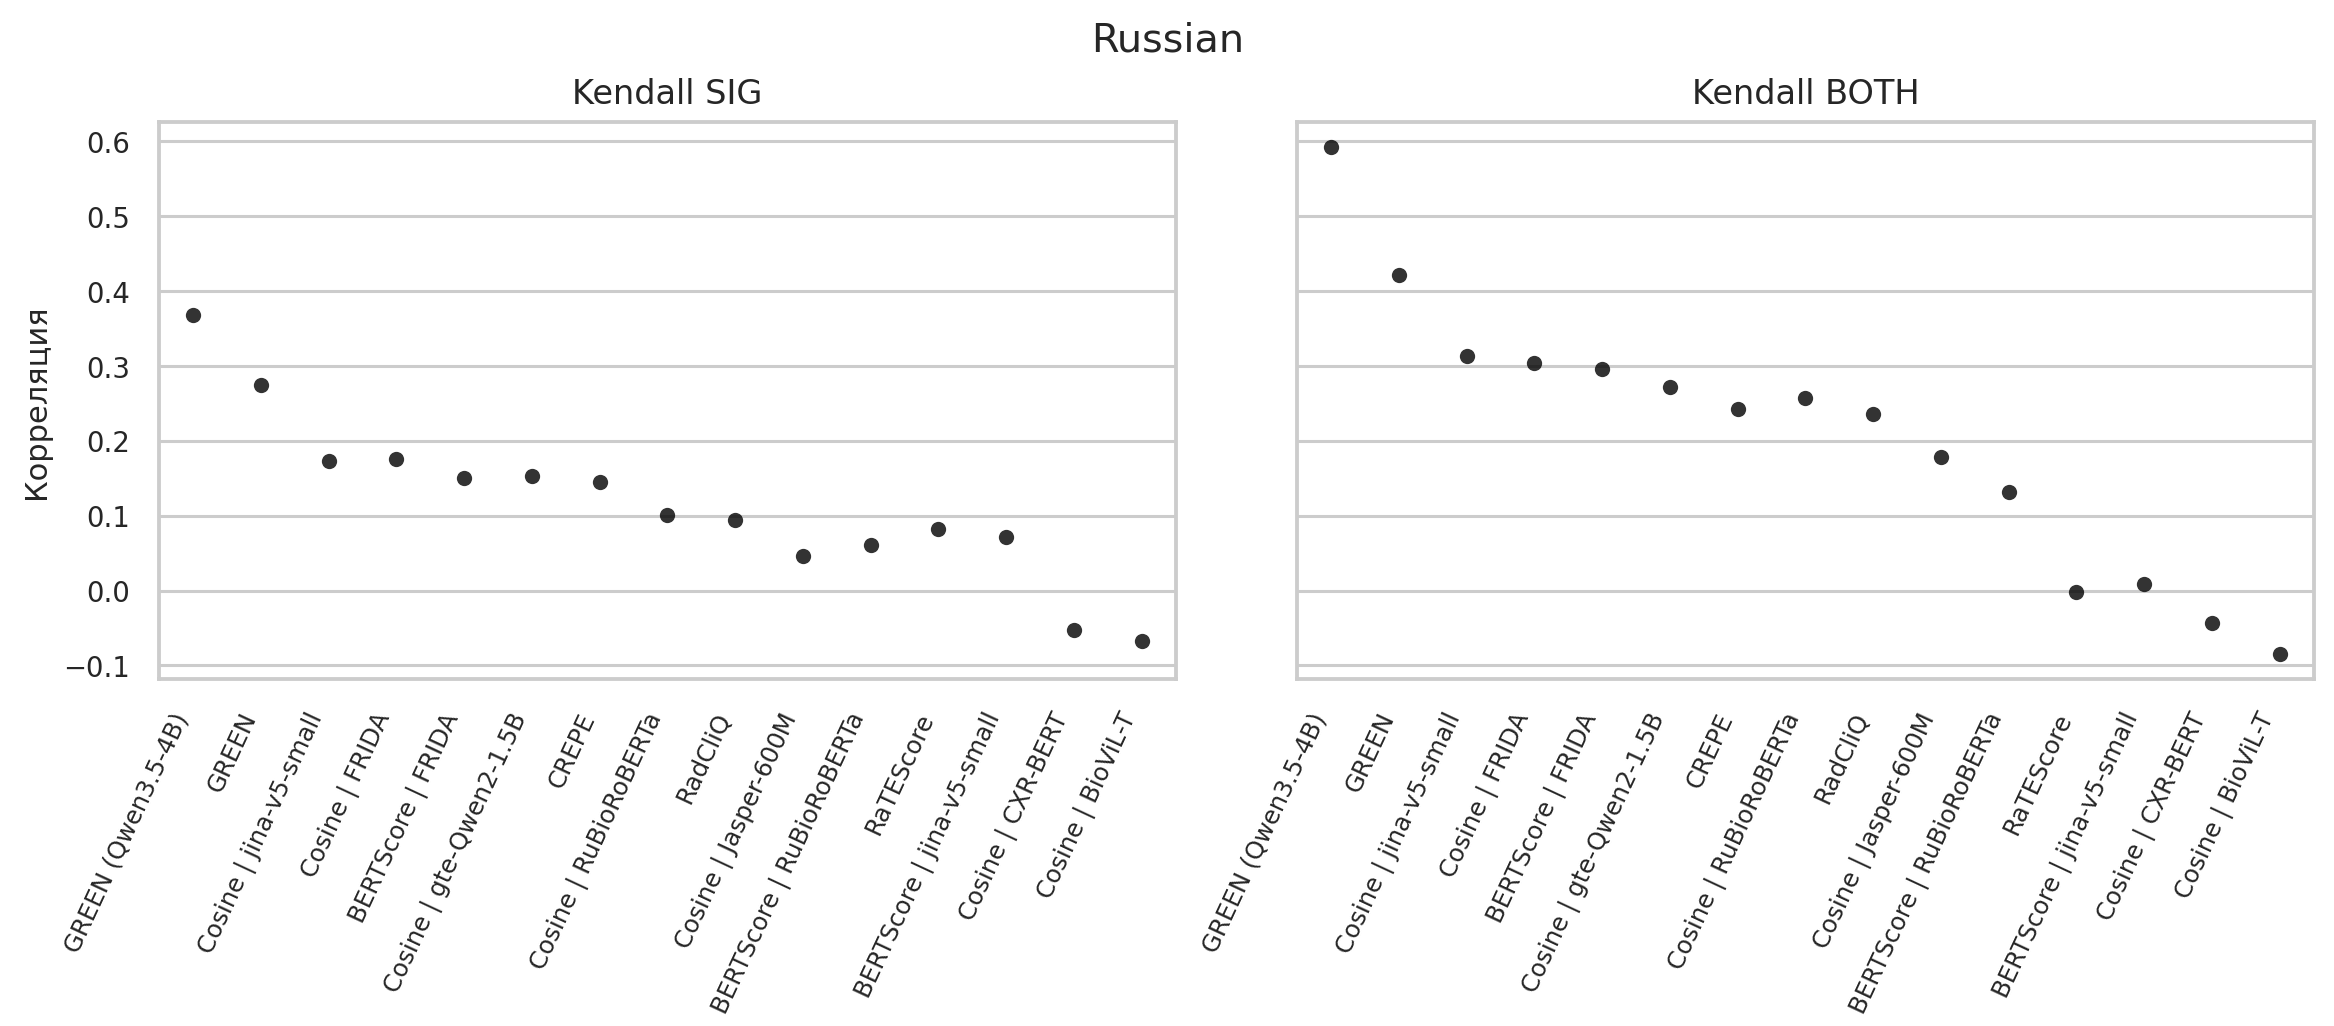
\includegraphics[width=\textwidth]{images/radevalx-correlation-russian.png}
        \caption{Корреляция Кендалла со значениями оценок на русском языке}
        \label{fig:image_a}
    \end{subfigure}
    
    \begin{subfigure}[b]{0.99\textwidth}
        \centering
        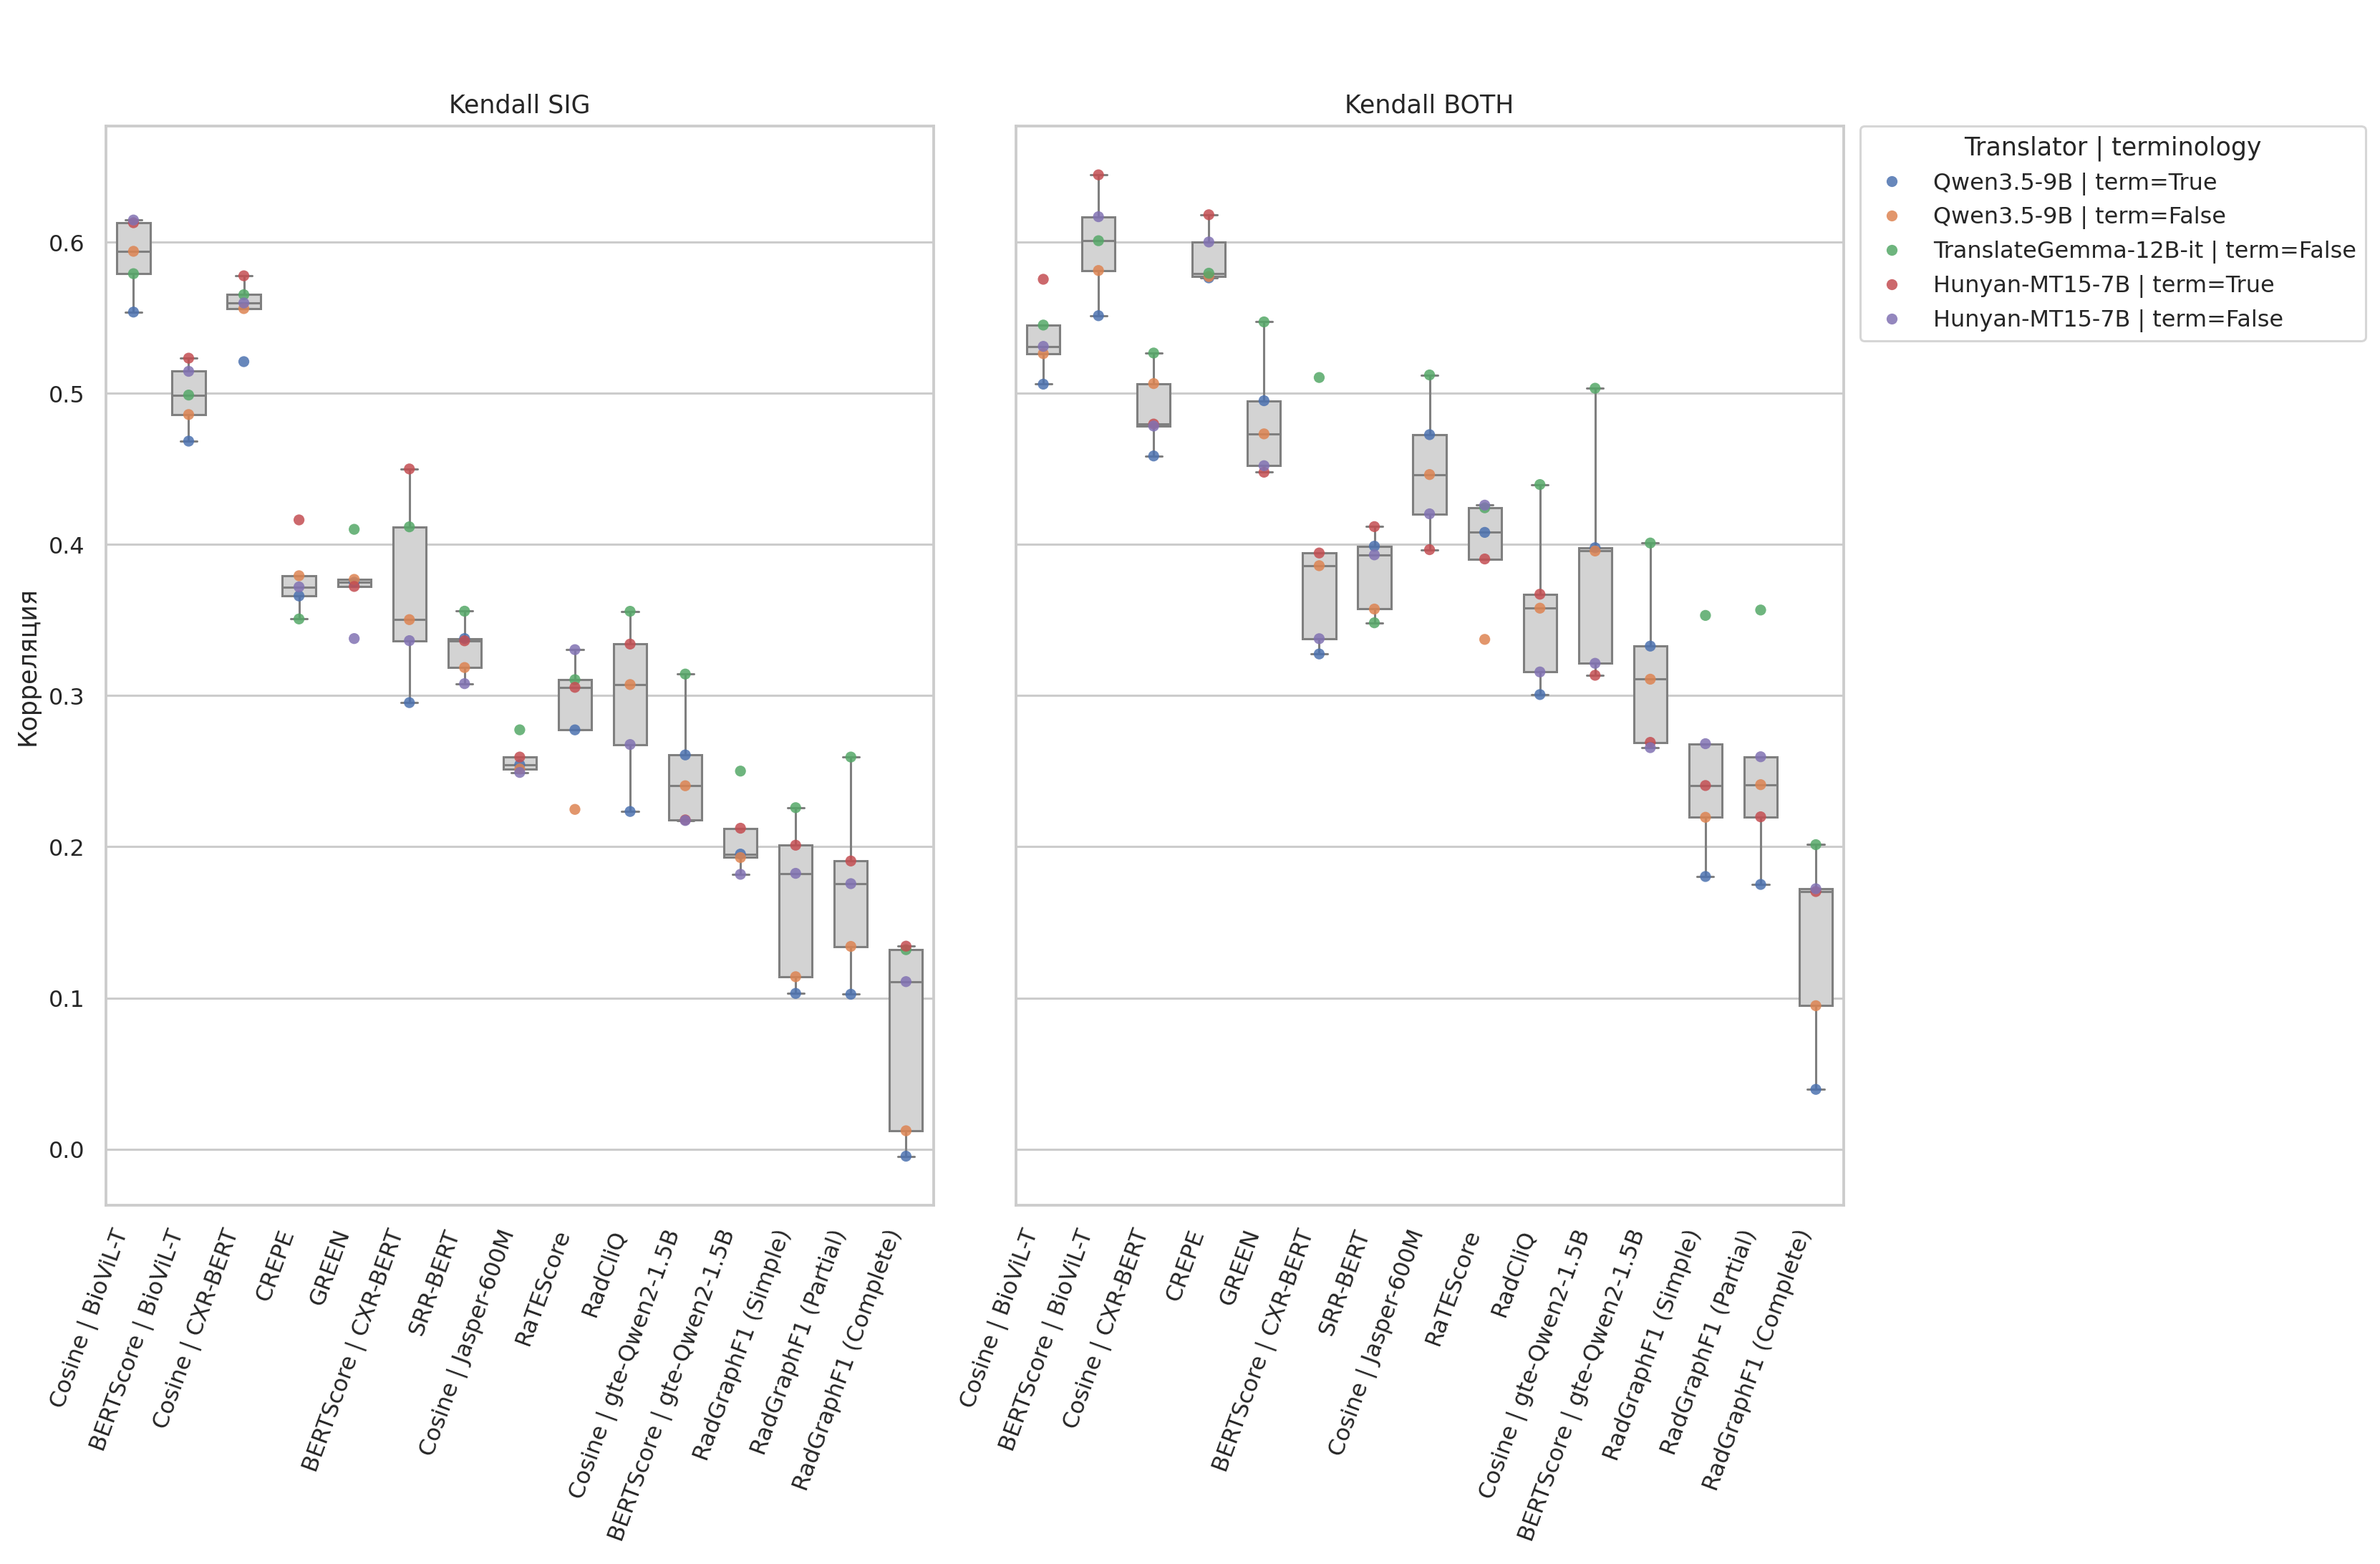
\includegraphics[width=\textwidth]{images/radevalx-correlation-english.png}
        \caption{Корреляция Кендалла со значениями оценок на английском языке}
        \label{fig:image_b}
    \end{subfigure}
    
    \caption{Сравнение коэффициентов корреляции Кендалла между значениями базовых оценок и числом ошибок на наборе данных RadEvalX. По оси абсцисс перечислены базовые способы оценки, по оси ординат -- коэффициент корреляции Кендалла. Цветные точки соответствуют различным моделям перевода и режимам использования терминологической таблицы. Слева в каждом подрисунке приведена корреляция с числом клинически значимых ошибок (SIG), справа -- с общим числом ошибок (BOTH).}
    \label{fig:radevalx-metric-corr}
\end{figure}

Русскоязычная клиническая компонента в работе строилась на основе подхода GREEN~\cite{ostmeier2024green}, адаптированного к русскоязычным радиологическим текстам. GREEN предназначен для сравнения кандидатного и эталонного заключений с акцентом на клинически значимые расхождения: ложные указания находок, пропуски, ошибки в локализации, степени выраженности и формулировках неопределённости. В рамках данной работы в русскоязычном варианте GREEN в качестве базовой языковой модели использовалась открытая модель Qwen3.5-9B~\cite{qwen3_5_technical_report} без дообучения на русскоязычных медицинских текстах. Ключевой особенностью данного решения является его интерпретируемость: помимо количественной оценки числа ошибок, метод предоставляет текстовое объяснение выявленных расхождений.

В качестве текстовых англоязычных компонент рассматривались подходы RadGraph, RadCliQ и RaTEScore, а также подходы на основе косинусной близости и BERTScore векторных представлений, полученных с помощью специализированных медицинских моделей CXR-BERT-specialized и BioViL-T~\cite{boecking2022making, bannur2023learning}. Подход RadGraph опирается на структурированное представление радиологического текста в виде графа сущностей и отношений~\cite{jain2021radgraph,delbrouck2022semanticrewards}. Для каждого заключения автоматически выделяются анатомические сущности, наблюдения и связи между ними, после чего кандидатный и эталонный тексты сравниваются на уровне совпадения клинически значимых объектов и их отношений.

Подход RadCliQ был предложен как составной показатель качества радиологических заключений, обученный так, чтобы согласоваться с экспертной оценкой рентгенологов~\cite{yu2023evaluating}. Он объединяет несколько англоязычных методов оценки, включая лексическое сходство, контекстную близость, близость по клиническим ярлыкам и структурное совпадение по RadGraph. В исходной постановке меньшие значения RadCliQ соответствуют лучшему качеству отчёта. Для согласования направления шкалы с остальными компонентами в данной работе использовалась величина
$\frac{1}{\mathrm{RadCliQ}}$, так что большее значение означало более высокое качество заключения-кандидата.

Подход RaTEScore ориентирован на сравнение радиологических текстов на уровне медицинских сущностей~\cite{zhao2024ratescore}. В его основе лежит предварительное выделение сущностей из радиологического текста с последующим сопоставлением их представлений в векторном пространстве.

Векторные представления, использованные в компонентах на основе косинусной близости и BERTScore, извлекались с помощью специализированной модели CXR-BERT-specialized~\cite{boecking2022making}. Она представляет собой текстовый кодировщик для радиологических текстов, построенный на основе базовой модели CXR-BERT, которая в свою очередь была обучена на специализированном словаре и корпусах предметной области. Модель CXR-BERT-specialized дополнительно обучалась в постановке согласования текста отчёта с одиночными рентгенограммами грудной клетки. 

Предобучение BioViL-T выполнялось на наборе MIMIC-CXR v2~\cite{mimic_cxr_dataset,mimic_cxr_scidata}, содержащем повторные рентгенологические исследования одних и тех же пациентов~\cite{bannur2023learning}. В обучающую выборку включались исследования с фронтальным снимком, для которых был доступен раздел заключения (Impression), при наличии предшествующего исследования дополнительно использовалось соответствующее предыдущее изображение. В результате формировалось объединение примеров двух типов: с одной рентгенограммой и с парой текущего и предыдущего изображений. Авторы указывают, что для предобучения было собрано $174.1$ тыс. обучающих и $4.9$ тыс. валидационных пар <<изображение-текст>>, причём большая часть обучающих примеров содержала предыдущее изображение.

По своей архитектуре BioViL-T является мультимодальной моделью, где визуальный кодировщик представляет собой гибрид сверточной нейронной сети и архитектуры Transformer, а текстовый -- кодировщик с архитектурой BERT, инициализированный весами базовой модели CXR-BERT~\cite{bannur2023learning}. На вход текстового кодировщика подается токенизированный (разбитый на токены -- минимальные текстовые единицы) радиологический текст. В процессе обучения данные проходят через модель дважды: первый проход выполняется с маскированием токенов для решения задачи языкового моделирования с опорой на визуальные данные, а второй -- без маскирования, для контрастивного выравнивания с визуальными представлениями. На финальном этапе текстовые и визуальные признаки отображаются в единое скрытое пространство для совместной оптимизации.

Косинусная близость рассчитывалась для векторных представлений текста заключения. Если $\mathbf{s}^{(c)}$ и $\mathbf{s}^{(r)}$ -- векторные представления текста-кандидата и текста-эталона соответственно, то соответствующая оценка вычислялась как
\[
\mathrm{CosSim}\!\left(\mathbf{s}^{(c)}, \mathbf{s}^{(r)}\right)
=
\frac{\left(\mathbf{s}^{(c)}\right)^{\top}\mathbf{s}^{(r)}}
{\left\|\mathbf{s}^{(c)}\right\|_2\,\left\|\mathbf{s}^{(r)}\right\|_2}.
\]

Для более детального сопоставления текстов на уровне токенов использовался подход BERTScore с использованием ранее упомянутых специализированных кодировщиков CXR-BERT-specialized и BioViL-T. В отличие от стандартной косинусной близости, оценивающей сходство текстов на макроуровне, данный метод предполагает вычисление аналогов точности и полноты за счёт нахождения наилучших попарных совпадений между контекстными векторными представлениями каждого токена кандидатного и эталонного отчётов.

Визуально-текстовые компоненты были включены в предлагаемый метод для того, чтобы итоговая оценка учитывала не только сходство с эталонным текстом, но и согласованность отчёта с изображением. Одной из таких компонент является BioViL-T~\cite{bannur2023learning}. Итоговая оценка сходства отчёта-кандидата с изображением получалась путём вычисления косинусной близости векторных представлений текста отчёта и снимка, полученных из кодировщика BioViL-T.

Дополнительно в рамках работы был обучен проектор, переводящий текстовые эмбеддинги, полученные моделью CXR-BERT-specialized, в общее визуально-текстовое пространство специализированного медицинского мультимодального кодировщика MedSigLIP. Для оптимизации модели использовалась попарная сигмоидная функция потерь, описанная в работе~\cite{zhai2023siglip} (архитектура SigLIP): каждая пара <<изображение-текст>> внутри мини-батча рассматривалась как отдельный бинарный пример, причём согласованные пары считались положительными, а несогласованные -- отрицательными.

Обучение выполнялось на наборе CheXpert Plus~\cite{chambon2024chexpertplus}. Данный набор данных содержит 223\,462 рентгенограмм грудной клетки из 187\,711 исследований 64\,725 пациентов. Каждому снимку соответствует текст радиологического отчёта, разбитый на разделы с помощью автоматической разметки, а также метаданные пациента, такие как пол, возраст и т. д. Для обучения проектора использовался текст из раздела заключение (Impression), полученный после первичной фильтрации набора данных, представляющей собой удаление слишком коротких (менее 10 слов) и повторяющихся отчётов. Пример изображения и соответствующего ему раздела заключения представлен на Рис.~\ref{fig:chexpertplus-example}.

\begin{figure}[h]
    \centering
    \small
    \setlength{\tabcolsep}{10pt}
    \renewcommand{\arraystretch}{1.25}

    \begin{tabular}{m{0.40\textwidth}m{0.50\textwidth}}
        \centering
        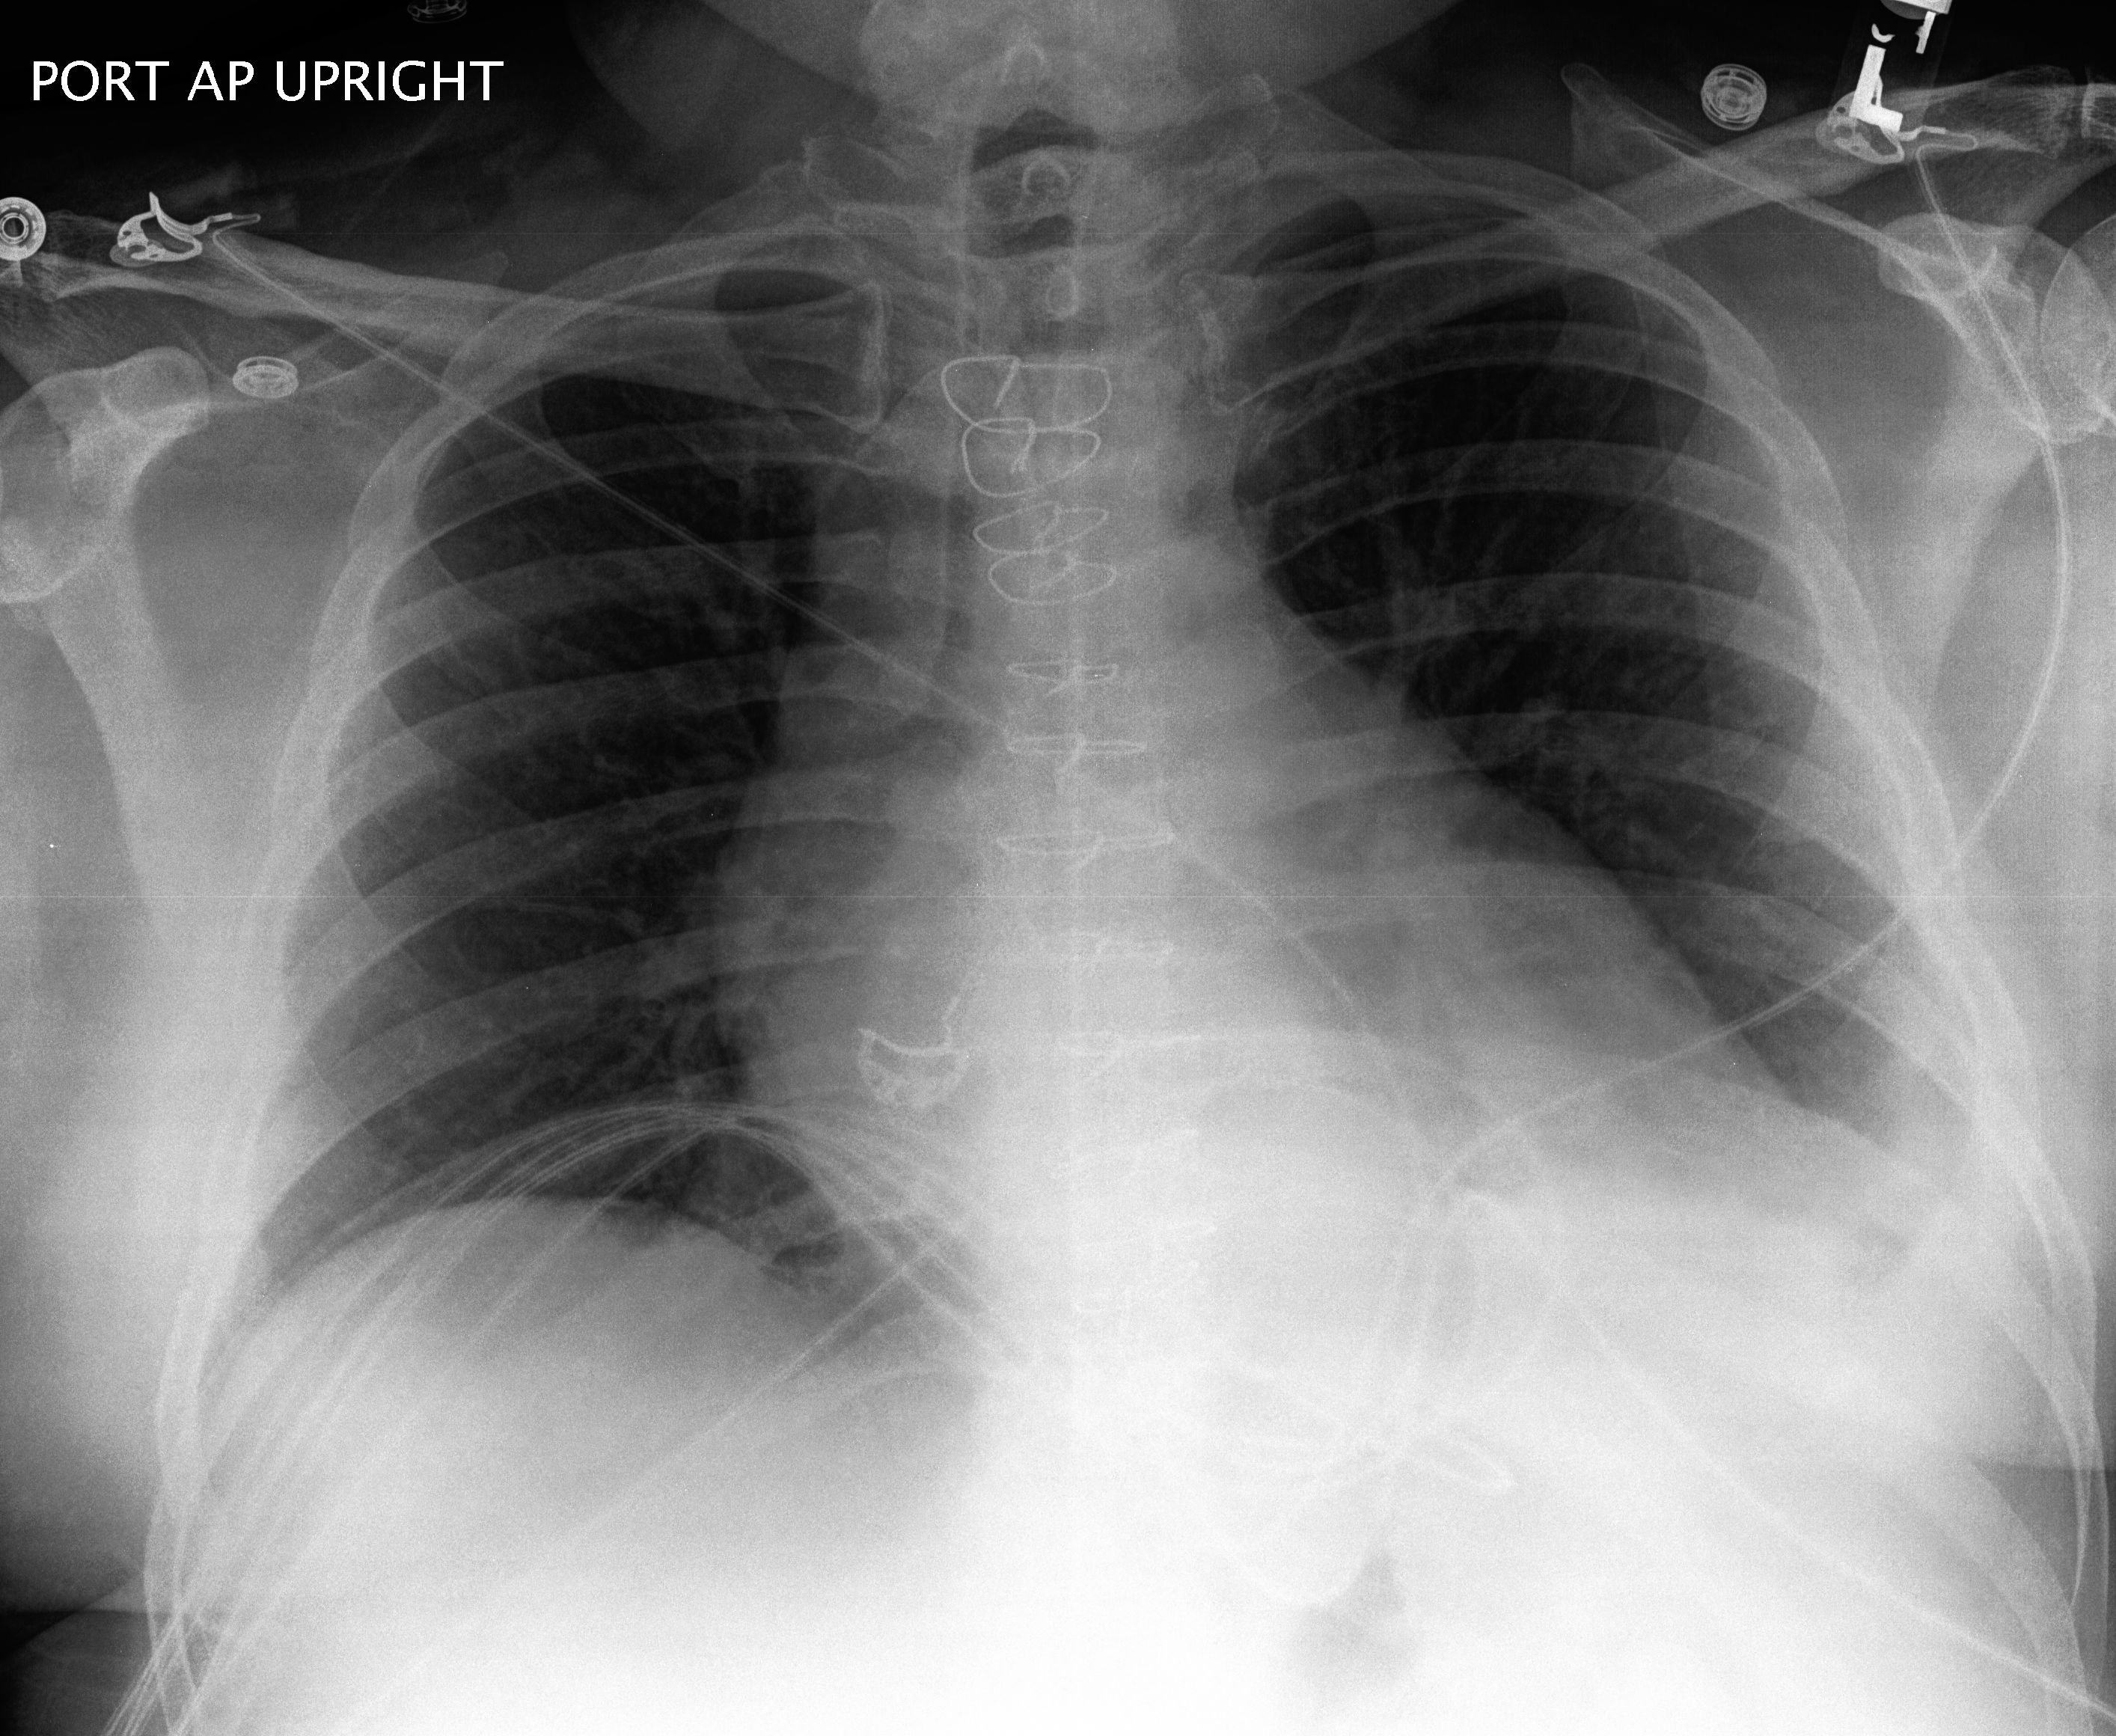
\includegraphics[width=\linewidth]{images/view1_frontal.png}
        &
        \textbf{Impression:}\par
        1. ENLARGEMENT OF CARDIO/PERICARDIAL SILHOUETTE AGAIN SEEN. VASCULAR REDISTRIBUTION IS NOTED; INCREASED LEFT RETROCARDIAC ATELECTASIS AND INCREASED SIZE OF LEFT-SIDED PLEURAL EFFUSION.\par
        2. FINDINGS CONSISTENT WITH PERSISTENT PULMONARY EDEMA WITH WORSENING LEFT RETROCARDIAC ATELECTASIS AND LEFT PLEURAL EFFUSION.
        \\
    \end{tabular}

    \caption{Пример пары снимка и отчёта (раздел Impression) из CheXpert Plus.}
    \label{fig:chexpertplus-example}
\end{figure}

Пусть $I_i$ обозначает изображение, а $T_i$ -- соответствующий ему текст отчёта. Для каждого объекта сначала строится векторное представление текста
\[
h_i = E_{\mathrm{CXR\text{-}BERT}}(T_i) \in \mathbb{R}^{d_{\mathrm{in}}},
\]
где $E_{\mathrm{CXR\text{-}BERT}}$ -- текстовый кодировщик CXR-BERT-specialized. Далее это представление подается на вход обучаемого проектора
\[
\tilde{y}_i = P_{\theta}(h_i) \in \mathbb{R}^{d_{\mathrm{out}}},
\]
где $P_{\theta}$ -- многослойный персептрон, отображающий эмбеддинг CXR-BERT-specialized в визуально-текстовое пространство MedSigLIP~\cite{sellergren2025medgemma}.

Проектор представляет собой полносвязную сеть с двумя скрытыми слоями. Он принимает на вход вектор $h \in \mathbb{R}^{d_{\mathrm{in}}}$ -- глобальное представление текста, извлечённое из CLS-токена. Далее применяется последовательность линейных преобразований с размерами слоёв
\[
d_{\mathrm{in}} \rightarrow 1024 \rightarrow 512 \rightarrow d_{\mathrm{out}},
\]
где \(d_{\mathrm{out}}\) совпадает с размерностью визуальных признаков MedSigLIP. Между внутренними линейными слоями используется функция активации GELU и регуляризация dropout (случайное зануление части признаков) с вероятностью \(0.1\).

Далее к визуальным и текстовым представлениям применяется $L_2$-нормализация:
\[
x_i = \frac{v_i}{\|v_i\|_2},
\qquad
y_i = \frac{\tilde{y}_i}{\|\tilde{y}_i\|_2},
\]
где $v_i$ -- векторное представление изображения $I_i$ в пространстве MedSigLIP, а $y_i$ -- нормированная проекция текстового эмбеддинга. Тогда попарное сходство между изображением $I_i$ и текстом $T_j$ определяется как скалярное произведение
\[
s_{ij} = x_i^\top y_j.
\]

Далее вводятся обучаемые скалярные параметры $t'$ и $b$, причём
\[
t = \exp(t').
\]
Тогда логит (линейный отклик перед применением сигмоиды) для пары $(I_i, T_j)$ равен
\[
\ell_{ij} = t\, x_i^\top y_j + b.
\]
Как и в оригинальной статье авторов SigLIP, параметр $t'$ отвечает за масштабирование сходства, а параметр $b$ компенсирует сильный дисбаланс между числом положительных и отрицательных пар в мини-батче (группе примеров, одновременно подаваемых модели).

Для мини-батча размера $|B|$ формируется матрица меток
\[
z_{ij} =
\begin{cases}
1, & i=j,\\
-1, & i\neq j,
\end{cases}
\]
то есть диагональные элементы соответствуют истинным парам <<изображение-текст>>, а все внедиагональные элементы -- отрицательным парам. Тогда попарная сигмоидная функция потерь записывается как
\[
\mathcal{L}_{\mathrm{SigLIP}}
=
-
\frac{1}{|B|}
\sum_{i=1}^{|B|}
\sum_{j=1}^{|B|}
\log \sigma\!\left(z_{ij}\left(t\,x_i^\top y_j + b\right)\right),
\]
где $\sigma(\cdot)$ -- функция сигмоиды.

С практической точки зрения обучение устроено следующим образом. Для каждого мини-батча берутся визуальные представления изображений в пространстве MedSigLIP и текстовые представления отчётов, полученные CXR-BERT-specialized. Далее обучаемый проектор $P_{\theta}$ преобразует текстовые эмбеддинги в то же пространство, после чего вычисляется попарная сигмоидная функция потерь по всем парам внутри батча. Минимизация этой функции приводит к тому, что проекция текста, соответствующего данному изображению, приближается к векторному представлению снимка, тогда как проекции остальных отчётов становятся дальше. В результате после обучения проектор реализует отображение
\[
P_{\theta} : \mathbb{R}^{d_{\mathrm{in}}} \to \mathbb{R}^{d_{\mathrm{out}}},
\]
согласующее текстовые представления, полученные с помощью кодировщика CXR-BERT-specialized, с визуально-текстовым пространством MedSigLIP.

После завершения обучения для пары <<снимок-отчёт>> можно вычислять согласованность между изображением и текстом как сходство
\[
\mathrm{score}_{\mathrm{img\text{-}text}}(I,T) = x^\top y,
\]
где $x$ -- нормированное векторное представление снимка, а $y$ -- нормированная проекция текстового векторного представления отчёта. Эта величина затем используется как базовая компонента в составе предлагаемого итогового способа оценки качества радиологического заключения.

\subsection{Кросс-валидация}

Пусть задан набор объектов
\[
D = \left\{(x_i, y_i)\right\}_{i=1}^{N},
\]
где $x_i$ -- $i$-я запись набора данных, включающая изображение, эталонный отчёт, кандидатный отчёт и вычисленные значения базовых оценочных сигналов, а $y_i$ -- целевая величина, характеризующая качество кандидатного отчёта. В данной работе в качестве целевой величины используется число клинически значимых ошибок в кандидатном заключении относительно эталона.

Каждая допустимая конфигурация $c \in \mathcal{C}$ задается выбором трёх компонент:
\begin{enumerate}
    \item русскоязычной клинической компоненты;
    \item одной текстовой компоненты;
    \item одной визуально-текстовой компоненты.
\end{enumerate}
Кроме того, конфигурация неявно включает используемый переводчик, поскольку англоязычные способы оценки вычисляются по английской версии отчётов. Для объекта $x_i$ и конфигурации $c$ формируется вектор признаков
\[
\mathbf{f}_i^{(c)} =
\left(
f^{(c)}_{\mathrm{ru},i},
f^{(c)}_{\mathrm{text},i},
f^{(c)}_{\mathrm{img},i}
\right).
\]

Поскольку значения различных компонент имеют разные масштабы, перед смешиванием выполняется стандартизация признаков. Для каждого признака $j \in \{\mathrm{ru}, \mathrm{text}, \mathrm{img}\}$ на обучающей части текущего разбиения выборки (фолда) вычисляются выборочное среднее $\mu_j$ и стандартное отклонение $\sigma_j$, после чего выполняется преобразование
\[
z^{(c)}_{j,i} = \frac{f^{(c)}_{j,i} - \mu_j}{\sigma_j}.
\]
Если для некоторого признака стандартное отклонение оказывается близким к нулю, то в реализации оно заменяется единицей, чтобы избежать деления на нуль. Вычисление параметров стандартизации по обучающей части соответствующего разбиения исключает утечку информации.

Итоговая оценка качества для объекта $x_i$ в конфигурации $c$ задается как линейная комбинация нормированных признаков:
\[
S_i^{(c,\mathbf{w})}
=
w_{\mathrm{ru}} z^{(c)}_{\mathrm{ru},i}
+
w_{\mathrm{text}} z^{(c)}_{\mathrm{text},i}
+
w_{\mathrm{img}} z^{(c)}_{\mathrm{img},i},
\]
где вектор весов $\mathbf{w} = \left(w_{\mathrm{ru}}, w_{\mathrm{text}}, w_{\mathrm{img}}\right)$ удовлетворяет ограничениям
\[
w_{\mathrm{ru}} > 0,\qquad
w_{\mathrm{text}} \ge 0,\qquad
w_{\mathrm{img}} > 0,\qquad
w_{\mathrm{ru}} + w_{\mathrm{text}} + w_{\mathrm{img}} = 1.
\]

Поскольку высокая оценка $S_i^{(c,\mathbf{w})}$ должна соответствовать более качественному отчёту, а большее значение $y_i$ соответствует большему числу ошибок, желаемая связь между ними является отрицательной. Поэтому в качестве целевой функции используется величина
\[
J(c,\mathbf{w}) = -\tau\!\left(S^{(c,\mathbf{w})}, y\right),
\]
где $\tau(\cdot,\cdot)$ -- коэффициент корреляции Кендалла между вектором итоговых оценок и вектором числа ошибок.

Ранговая корреляция Кендалла широко используется в работах по оценке качества радиологических отчётов при сопоставлении автоматических оценочных сигналов с врачебной оценкой. Кроме того, ранговый характер коэффициента делает его менее чувствительным к единичным выбросам и не требует предположения о нормальности распределения или линейности связи. Коэффициент корреляции Кендалла задаётся следующим образом:
\[
\tau =
\frac{N_{\text{согл}} - N_{\text{несогл}}}
{n(n-1)/2},
\]
где \(n\) -- число объектов, \(N_{\text{согл}}\) -- число согласованных пар объектов, а \(N_{\text{несогл}}\) -- число несогласованных пар. Знаменатель \(n(n-1)/2\) равен общему числу всех попарных сравнений между объектами. Пара объектов \(i\) и \(j\) считается согласованной, если
\[
\bigl(S_i^{(c,\mathbf{w})} - S_j^{(c,\mathbf{w})}\bigr)\bigl(y_i - y_j\bigr) > 0,
\]
и несогласованной, если
\[
\bigl(S_i^{(c,\mathbf{w})} - S_j^{(c,\mathbf{w})}\bigr)\bigl(y_i - y_j\bigr) < 0.
\]

Подбор весов осуществляется перебором по сетке на двухмерном симплексе. Пусть шаг сетки равен $h$. Тогда множество допустимых весов имеет вид
\[
\mathcal{W}_h =
\Bigl\{
\mathbf{w} \in \mathbb{R}^3
\Bigm|
\begin{aligned}
&w_{\mathrm{ru}}, w_{\mathrm{img}} > 0;\; w_{\mathrm{text}} \ge 0; \\
&w_{\mathrm{ru}} + w_{\mathrm{text}} + w_{\mathrm{img}} = 1;\;
w_{\mathrm{ru}}, w_{\mathrm{text}}, w_{\mathrm{img}} \in h\mathbb{Z}
\end{aligned}
\Bigr\}.
\]

Для корректной оценки качества не одной фиксированной конфигурации, а всей процедуры её выбора в работе используется вложенная кросс-валидация. Внешний цикл разбивает набор данных на $K_{\mathrm{outer}}$ фолдов. На каждом шаге один внешний фолд используется как тестовый, а остальные $K_{\mathrm{outer}}-1$ фолдов -- как внешняя обучающая часть. Именно на этой внешней обучающей части выполняется выбор конфигурации и подбор весов.

Внутри каждого внешнего шага запускается внутренний цикл из $K_{\mathrm{inner}}$ фолдов. Для каждой конфигурации $c \in \mathcal{C}$ и для каждого внутреннего разбиения последовательно выполняются следующие действия:
\begin{enumerate}
    \item на внутренней обучающей части вычисляются параметры стандартизации;
    \item на этой же части перебором по множеству $\mathcal{W}_h$ выбирается вектор весов
    \[
    \mathbf{w}^{*}
    =
    \arg\max_{\mathbf{w}\in\mathcal{W}_h}
    J_{\mathrm{train}}(c,\mathbf{w});
    \]
    \item найденные параметры стандартизации и веса переносятся на внутреннюю валидационную часть;
    \item на валидационной части вычисляется значение
    \[
    J_{\mathrm{val}}(c,\mathbf{w}^{*}).
    \]
\end{enumerate}

После прохождения всех внутренних фолдов для каждой конфигурации вычисляется среднее значение
\[
\overline{J}_{\mathrm{inner}}(c)
=
\frac{1}{K_{\mathrm{inner}}}
\sum_{\ell=1}^{K_{\mathrm{inner}}}
J_{\mathrm{val}}^{(\ell)}(c)
\]
и стандартное отклонение этой величины по внутренним фолдам. В качестве лучшей выбирается конфигурация
\[
c^{*}
=
\arg\max_{c \in \mathcal{C}}
\overline{J}_{\mathrm{inner}}(c).
\]

После выбора лучшей конфигурации $c^{*}$ по внешней обучающей части выборки заново пересчитываются параметры стандартизации и снова перебором по сетке находится оптимальный вектор весов
\[
\mathbf{w}^{*}_{\mathrm{outer}}
=
\arg\max_{\mathbf{w}\in\mathcal{W}_h}
J_{\mathrm{outer\_train}}(c^{*},\mathbf{w}).
\]
Затем найденные параметры применяются к внешнему тестовому фолду, и на нем вычисляется итоговое значение
\[
J_{\mathrm{outer\_test}} = -\tau\!\left(S_{\mathrm{outer\_test}}, y_{\mathrm{outer\_test}}\right).
\]

Описанная процедура повторяется для всех внешних фолдов. В результате получается набор внешних оценок
\[
J_1, J_2, \dots, J_{K_{\mathrm{outer}}},
\]
по которым далее вычисляются среднее значение, стандартное отклонение и доверительный интервал.

% \subsection{Программная реализация подхода}

% Описанная процедура была реализована в виде Python-скрипта, который принимает на вход таблицу в формате CSV с заранее вычисленными значениями базовых оценочнок и целевой переменной. Реализация организована таким образом, чтобы воспроизводить полный цикл эксперимента: от подготовки данных и построения допустимых конфигураций до проведения вложенной кросс-валидации и сохранения итоговых результатов.

% На этапе загрузки и предварительной обработки данных скрипт проверяет наличие обязательных столбцов, включая целевую переменную --- число ошибок --- и русскоязычный клинический сигнал. Далее автоматически определяются все текстовые столбцы вида \texttt{text\_en\_*} и все визуально-текстовые столбцы вида \texttt{img\_en\_*}. После этого выполняется очистка данных: удаляются строки с пропусками в обязательных полях, значения приводятся к числовому виду, а для каждой строки выбирается идентификатор \texttt{row\_id}. Если в исходной таблице отсутствует специальный идентификатор, он формируется автоматически на основе индекса строки.

% Следующим этапом является построение допустимых конфигураций. Каждая конфигурация должна использовать согласованные текстовый и визуально-текстовый сигналы. Для этого в именах столбцов выделяется общий суффикс, соответствующий конкретному переводчику и режиму его работы. Иными словами, текстовый и визуально-текстовый сигналы объединяются в одну конфигурацию только в том случае, если они были рассчитаны для одной и той же английской версии отчётов. Такой шаг необходим для корректного сравнения, поскольку использование текстового сигнала, вычисленного для одного перевода, совместно с визуально-текстовым сигналом, вычисленным для другого перевода, привело бы к методологически некорректной смеси.

% После формирования множества конфигураций скрипт строит сетку допустимых весов на симплексе. Пользователь задает шаг \texttt{weight\_step}, после чего автоматически перечисляются все тройки неотрицательных весов, сумма которых равна единице. Например, при шаге $0.05$ перебираются все комбинации вида
% \[
% (w_{\mathrm{ru}}, w_{\mathrm{text}}, w_{\mathrm{img}})
% \]
% такие, что каждое значение кратно $0.05$, неотрицательно, а сумма трёх значений равна единице. Благодаря малому числу смешиваемых сигналов такой полный перебор остаётся вычислительно приемлемым и позволяет избежать нестабильности, которая могла бы возникнуть при использовании градиентных процедур на очень малых выборках.

% Основная часть реализации сосредоточена в процедуре вложенной кросс-валидации. Для каждого внешнего фолда формируется внешняя обучающая и внешняя тестовая часть. Далее для каждой допустимой конфигурации выполняется внутренний цикл: на каждом внутреннем обучающем подмножестве вычисляются параметры стандартизации, на нем же перебором по сетке подбираются веса, после чего выбранные параметры переносятся на внутреннее валидационное подмножество. Полученные значения целевой функции усредняются по внутренним фолдам, и по этому среднему выбирается наилучшая конфигурация. Затем на всей внешней обучающей части для выбранной конфигурации повторно оцениваются параметры стандартизации и подбираются веса, после чего итоговая оценка качества вычисляется на внешнем тестовом фолде.

% С практической точки зрения важным элементом реализации является журналирование всех промежуточных результатов. Скрипт сохраняет подробный лог внутренней и внешней кросс-валидации, содержащий информацию о выбранной конфигурации, найденных весах, размере обучающей, валидационной и тестовой частей, а также о значениях целевой функции на каждом шаге. Отдельно сохраняются итоговые оценки для всех объектов внешних тестовых фолдов, что позволяет впоследствии строить графики и выполнять дополнительный анализ.

% Кроме табличных результатов, скрипт автоматически формирует сводные файлы и визуализации. К числу сохраняемых результатов относятся:
% \begin{enumerate}
%     \item полный журнал кросс-валидации;
%     \item таблица итоговых внешних предсказаний;
%     \item таблица результатов по внешним фолдам;
%     \item итоговая сводка в форматах \texttt{JSON} и \texttt{CSV};
%     \item графики, иллюстрирующие разброс качества по фолдам, распределение весов и связь итоговой оценки с числом ошибок.
% \end{enumerate}

% Тем самым программная реализация отражает не только вычислительную сторону предлагаемого подхода, но и его исследовательскую логику. Скрипт реализует полный воспроизводимый пайплайн, в котором автоматически выполняются очистка данных, формирование конфигураций, подбор весов, выбор наилучшего сочетания компонентов и итоговая оценка качества на основе вложенной кросс-валидации. Это позволяет рассматривать его как практическое воплощение предложенного в работе способа оценки качества русскоязычных радиологических отчётов.